\section{Bayesian Analysis Toolkit} \label{sec:fit:bat}

The Bayesian Analysis Toolkit (BAT) \cite{Beaujean:2011zz,Beresford:2642397} is
used to obtain the marginalized posterior distribution in \Cref{eq:fit:bayes}
discussed in \Cref{sec:fit:theory}.  It takes as input the data, the parameters
$\nu$ and $\boldsymbol{\theta}$ along with their corresponding prior
distributions discussed in \Cref{sec:fit:priors}, and the chosen likelihood
function $\mathcal{L}(\nu,\boldsymbol{\theta}|\text{data})$.  Here the
likelihood function is given by the product of the Poisson probability in each
bin: 

\begin{equation} \label{sec:fit:likelihood}
\mathcal{L}(\nu,\boldsymbol{\theta}|\text{data}) = \prod_{i=1}^{N} \frac{(s_{i}(\nu,\boldsymbol{\theta}) + b_{i}(\nu,\boldsymbol{\theta}))^{n_{i}}}{n_{i}!} e^{-(s_{i}(\nu,\boldsymbol{\theta}) + b_{i}(\nu,\boldsymbol{\theta}))}
\end{equation}

In the above the product runs over all $N$ bins in the histogram being fit,
$s_{i}$ and $b_{i}$ are the expected number of signal and background events
expected in bin $i$ dependent upon $\nu$ and $\boldsymbol{\theta}$, and $n_{i}$
is the number of data events in bin $i$.  Note that in \Cref{sec:fit:priors}
the signal parameter priors are normalized to unity such that $\nu$ corresponds
to the number of signal events. Now \Cref{sec:fit:likelihood} can be used to
calculate the probability of a given set of parameter values $\nu$ and
$\boldsymbol{\theta}$ given the data.  Plugging this definition into
\Cref{eq:fit:bayes} gives the final form of Bayes' equation used to
calculate the marginalized posterior $p(\nu|\text{data})$ given below.
%
\begin{equation} \label{sec:fit:full_bayes}
p(\nu|\text{data}) \propto \pi(\nu) \int \prod_{i=1}^{N} \frac{(s_{i}(\nu,\boldsymbol{\theta}) + b_{i}(\nu,\boldsymbol{\theta}))^{n_{i}}}{n_{i}!} e^{-(s_{i}(\nu,\boldsymbol{\theta}) + b_{i}(\nu,\boldsymbol{\theta}))} \prod_{j}\pi(\theta_j)\text{d}\boldsymbol{\theta}
\end{equation}

The final step is to calculate the integral in \Cref{sec:fit:full_bayes} across
the multi-dimensional space of $(\nu,\boldsymbol{\theta})$. However, calculating the
integral for such a large space is not computationally feasible, so BAT instead
employs a Markov Chain Monte Carlo (MCMC) \cite{2017arXiv170102434B,
Beresford:2642397} in order to sample the space efficiently.

The basic idea of a MCMC is to perform a random walk in the parameter space
$(\nu,\boldsymbol{\theta})$ making sure to spend more time sampling regions of
high probability, i.e sampling proportional to the posterior.  The sequence of
parameter values on the walk depends only on the previous set making the
resulting sequence of parameter values a Markov Chain \cite{Markov2006}.  The
Metropolis-Hastings algorithm \cite{10.2307/2334940,Beresford:2642397} is used
to generate the Markov Chains used in BAT.  This procedure is detailed below
and an illustration of the process for only two parameters $\theta_{1}$ and
$\theta_{2}$ is shown in \Cref{sec:fit:markov_chain}.
%
\begin{enumerate}
\item The chain begins at position $\boldsymbol{x_{1}}$ in the parameter space to be sampled.
\item The next position, $\boldsymbol{x_{2}}$, is proposed by selecting each new parameter from a Breit-Wigner distribution centered on the value of the corresponding parameter for the current position $\boldsymbol{x_{1}}$.
\item A random number $r$ between 0 and 1 is selected from a uniform distribution.
\item The value of the posterior $p(\nu,\boldsymbol{\theta}|\text{data})$, given in \Cref{eq:fit:posterior}, is calculated for both  $\boldsymbol{x_{1}}$ and  $\boldsymbol{x_{2}}$ resulting in $p(\nu,\boldsymbol{\theta}|\text{data})_{1}$ and $p(\nu,\boldsymbol{\theta}|\text{data})_{2}$.
\item If $r < \frac{p(\nu,\boldsymbol{\theta}|\text{data})_{2}}{p(\nu,\boldsymbol{\theta}|\text{data})_{1}}$, the algorithm transitions to the new position $\boldsymbol{x_{2}}$ and it is added to the chain. Otherwise the algorithm remains at $\boldsymbol{x_{1}}$ and is added to the chain.
\item This process is then repeated starting from the chosen position defined as position $\boldsymbol{x_{1}}$.
\end{enumerate}

\begin{figure}[!htbp]
\centering
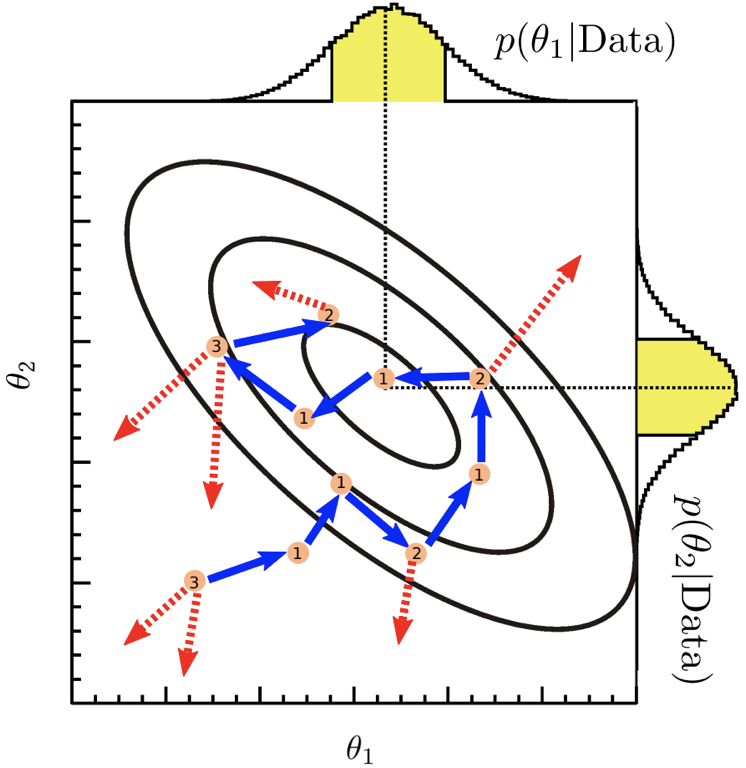
\includegraphics[width=0.7\linewidth]{figures/fit/markov_chain}
\caption{This figure illustrates a random walk in parameter space $(\theta_{1},\theta_{2})$. The numbers indicate the number of iterations the chain remained at this point in parameter space, the blue arrows indicate accepted transitions, and the red arrows indicate rejected transitions. The marginalized posterior distributions obtained for the two parameters $p(\theta_{1}|\text{data})$ and $p(\theta_{2}|\text{data})$ are also shown, and the yellow bands correspond to the central 68\% of the distributions \cite{Beresford:2642397}.}
\label{sec:fit:markov_chain}
\end{figure}

This random walk in parameter space generates a chain which preferentially
transitions to positions corresponding to high probability regions of the
posterior, effectively sampling the important regions of the posterior
distribution.  By plotting the frequency of occurrence for each parameter along
the chain, and then normalizing the distribution to unity, the desired
marginalized posterior for the signal parameter $p(\nu|\text{data})$ is found.
The mode of this marginalized posterior, known as the maximum a posteriori
probability (MAP), is used as the measured number of signal events ($\nu$) and
the standard deviation ($\sigma$) is used as the uncertainty on the
measurement. Dividing $\nu \pm \sigma$ by $(\mathcal{L}_{D} \times
\sigma_\text{H} \times \Gamma_{H \rightarrow b\bar{b}} \times
\text{A}_{s})$~\footnote{$\mathcal{L}_{D}$ is the luminosity of the dataset.
$\sigma_\text{H}$ is the cross section for the boosted Higgs boson production
production mechanism.  $\Gamma_{H \rightarrow b\bar{b}}$ is the branching fraction of the
Higgs boson to $b\bar{b}$. $\text{A}_{s}$ is the signal acceptance of event selection.}
the signal strength $\mu_{s} \pm \sigma_{s}$ is found.
